\documentclass[12pt,a4paper]{article}

\usepackage[margin=0.9in]{geometry}
\usepackage{amsmath,amssymb}
\usepackage{booktabs}
\usepackage{tabularx}
\usepackage{enumitem}
\usepackage{hyperref}
\usepackage{xcolor}
\usepackage{fancyhdr}
\usepackage{tikz}
\usepackage{tcolorbox}

\usetikzlibrary{arrows.meta,positioning,matrix}
\tcbuselibrary{skins,breakable}

% Neutral palette for formal academic presentation
\definecolor{primary}{RGB}{0,0,0}
\definecolor{secondary}{RGB}{60,60,60}
\definecolor{accent}{RGB}{85,85,85}
\definecolor{highlight}{RGB}{110,110,110}
\definecolor{danger}{RGB}{140,140,140}
\definecolor{light}{RGB}{245,245,245}

\hypersetup{
    hidelinks,
    pdftitle={Four Types of Artificial Intelligence Approaches},
    pdfauthor={Department of Computing}
}

\pagestyle{fancy}
\fancyhf{}
\lhead{Artificial Intelligence Foundations}
\rhead{Four Classical AI Approaches}
\rfoot{Page \thepage}

\setlength{\parskip}{0.5em}
\setlength{\parindent}{0pt}
\setlength{\headheight}{15pt}

\newtcolorbox{typebox}[1]{
    colback=light,
    colframe=primary,
    title=#1,
    fonttitle=\bfseries,
    rounded corners,
    boxrule=0.9pt,
    breakable
}

\newtcolorbox{examplebox}{
    colback=accent!10,
    colframe=accent,
    title=Example,
    fonttitle=\bfseries,
    rounded corners,
    boxrule=0.9pt,
    breakable
}

\newtcolorbox{insightbox}{
    colback=highlight!10,
    colframe=highlight,
    title=Key Insight,
    fonttitle=\bfseries,
    rounded corners,
    boxrule=0.9pt,
    breakable
}

\begin{document}

\begin{titlepage}
\centering
\vspace*{0.5cm}
{\Large\color{primary}\textbf{Academic Report}}\\[0.3cm]
\rule{\textwidth}{1.8pt}\\[0.5cm]
{\Huge\bfseries\color{primary}Four Types of Artificial Intelligence Approaches}\\[0.2cm]
{\Large Thinking Humanly, Thinking Rationally, Acting Humanly, Acting Rationally}\\[0.4cm]
\rule{\textwidth}{1.8pt}\\[1.0cm]

\begin{tabular}{rl}
\textbf{Topic:} & Introduction to foundational AI viewpoints \\
\textbf{Objective:} & Explain each type with practical examples \\
\textbf{Based On:} & Classical AI categorization framework \\
\textbf{Prepared On:} & \today
\end{tabular}

\vfill
{\large Department of Computing}\\
{\large Academic Notes}
\end{titlepage}

\tableofcontents
\newpage

\section{Introduction}

Artificial Intelligence is defined in different ways depending on what we expect from a machine.
A well-known framework groups AI definitions into four categories:
\begin{itemize}[noitemsep]
    \item Systems that think like humans
    \item Systems that think rationally
    \item Systems that act like humans
    \item Systems that act rationally
\end{itemize}

These four viewpoints can be understood using two axes:
\begin{itemize}[noitemsep]
    \item \textbf{Thinking vs Acting}
    \item \textbf{Human-like vs Rational (ideal) behavior}
\end{itemize}

\section{2x2 Framework Diagram}

\begin{figure}[h!]
\centering
\resizebox{0.95\textwidth}{!}{%
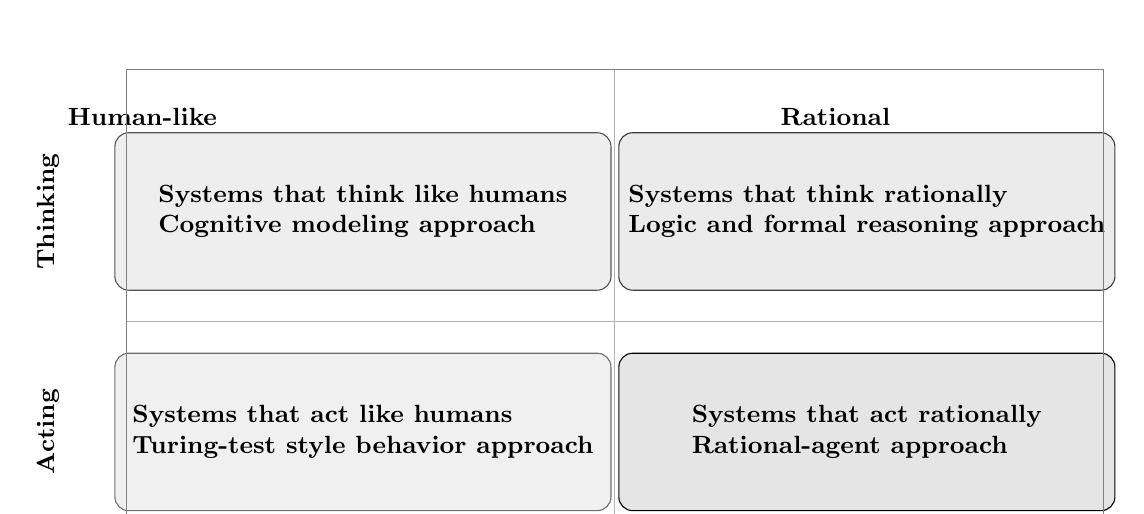
\begin{tikzpicture}[
    node distance=0.45cm,
    box/.style={rectangle, rounded corners=5pt, draw=#1, fill=#1!10, minimum width=6.3cm, minimum height=2.0cm, align=left, font=\small\bfseries},
    axislabel/.style={font=\small\bfseries}
]

% Axis labels
\node[axislabel] at (0,3.0) {Human-like};
\node[axislabel] at (8.8,3.0) {Rational};
\node[axislabel,rotate=90] at (-1.2,1.8) {Thinking};
\node[axislabel,rotate=90] at (-1.2,-1.0) {Acting};

% Grid boxes
\node[box=accent] (thuman) at (2.8,1.8) {Systems that think like humans\\Cognitive modeling approach};
\node[box=secondary] (trational) at (9.2,1.8) {Systems that think rationally\\Logic and formal reasoning approach};
\node[box=highlight] (ahuman) at (2.8,-1.0) {Systems that act like humans\\Turing-test style behavior approach};
\node[box=primary] (arational) at (9.2,-1.0) {Systems that act rationally\\Rational-agent approach};

% Thin frame around matrix
\draw[black!50] (-0.2,3.6) rectangle (12.2,-2.2);
\draw[black!30] (6.0,3.6) -- (6.0,-2.2);
\draw[black!30] (-0.2,0.4) -- (12.2,0.4);

\end{tikzpicture}
}
\caption{Classical four-category view of AI definitions.}
\label{fig:four-ai}
\end{figure}

\section{Systems That Think Like Humans}

\begin{typebox}{Definition}
This approach builds systems that imitate how humans \textit{actually think}.
The focus is not only correct output, but also a human-like thought process.
Researchers use ideas from cognitive psychology and neuroscience.
\end{typebox}

\textbf{Main objective:} Model human mental processes such as memory limits, attention, and step-by-step reasoning.

\begin{examplebox}
\textbf{Example: Intelligent Tutoring System}

Suppose a math learning platform wants to understand why a student repeatedly makes a fraction mistake.
A human-like thinking AI can model typical student misconceptions (for example, adding numerators and denominators directly).
Instead of only giving the right answer, it diagnoses the cognitive error pattern and gives feedback similar to a human teacher.
\end{examplebox}

\textbf{Strength:} Useful when we want interpretable, human-compatible explanations.

\textbf{Limitation:} Human thinking is often biased or inconsistent, so copying it exactly may not produce optimal decisions.

\section{Systems That Think Rationally}

\begin{typebox}{Definition}
This approach is based on the "laws of thought": use formal logic to derive correct conclusions from known facts.
A system is good if its reasoning is logically valid.
\end{typebox}

\textbf{Main objective:} Represent knowledge as symbols and rules, then apply inference to prove or derive conclusions.

\begin{examplebox}
\textbf{Example: Rule-Based Medical Expert System}

Imagine a knowledge base with rules such as:
\begin{itemize}[noitemsep]
    \item If fever and persistent cough, then possible respiratory infection.
    \item If respiratory infection and low oxygen, then high-risk case.
\end{itemize}
Given patient facts, the system uses logical inference to conclude risk category.
The process emphasizes correctness of reasoning rather than human-like conversation style.
\end{examplebox}

\textbf{Strength:} Precise and mathematically clean reasoning.

\textbf{Limitation:} Real-world environments are uncertain; pure logic can struggle with noisy, incomplete, or probabilistic data.

\section{Systems That Act Like Humans}

\begin{typebox}{Definition}
This approach focuses on behavior.
If a system behaves similarly to a human in conversation, perception, and interaction, it is considered intelligent.
This is related to the idea behind the Turing Test.
\end{typebox}

\textbf{Main objective:} Produce human-like observable behavior, especially in communication tasks.

\begin{examplebox}
\textbf{Example: Customer Support Chat Assistant}

A chatbot on an online store answers order queries, asks clarification questions, and responds politely in natural language.
If users cannot easily distinguish its responses from those of a human support agent, it performs well under the acting-humanly view.
\end{examplebox}

\textbf{Strength:} Strong user experience in interactive applications.

\textbf{Limitation:} Human-like behavior can hide weak internal reasoning; sounding natural does not always mean being correct.

\section{Systems That Act Rationally}

\begin{typebox}{Definition}
This is the modern dominant AI view.
A rational agent chooses actions that maximize expected success (or utility) based on available information.
The agent does not need to think exactly like a human.
\end{typebox}

\textbf{Main objective:} Select the best action in the current state to achieve goals under constraints.

A simple utility formulation is:
\begin{equation}
\pi^*(s) = \arg\max_{a \in A} \mathbb{E}[U(s,a)],
\end{equation}
where $\pi^*(s)$ is the best action policy in state $s$.

\begin{examplebox}
\textbf{Example: Autonomous Vacuum Robot}

A robot vacuum observes room layout, battery level, and dirt probability.
It plans movement to clean maximum area while avoiding collisions and ensuring it can return to the charging dock.
Its behavior is judged by effectiveness, not by whether it behaves like a human cleaner.
\end{examplebox}

\textbf{Strength:} Practical and performance-oriented for real-world systems.

\textbf{Limitation:} Requires good state estimation, reward design, and robust handling of uncertainty.

\section{Comparison Table}

\begin{center}
\small
\begin{tabularx}{\textwidth}{>{\bfseries}l X X}
\toprule
Approach & Success Criterion & Typical Use \\
\midrule
Think like humans & Match human cognitive process & Tutoring systems, cognitive simulation \\
Think rationally & Logical correctness of inference & Formal expert systems, theorem proving \\
Act like humans & Human-like external behavior & Conversational assistants, social robots \\
Act rationally & Goal achievement under constraints & Robotics, planning, autonomous systems \\
\bottomrule
\end{tabularx}
\end{center}

\section{One Problem Viewed in Four Ways}

Consider an AI assistant for study planning:
\begin{itemize}
    \item \textbf{Think humanly:} Mimics how students mentally prioritize tasks and forget deadlines.
    \item \textbf{Think rationally:} Uses strict logical rules to derive the best schedule from constraints.
    \item \textbf{Act humanly:} Talks like a human mentor and gives natural, empathetic suggestions.
    \item \textbf{Act rationally:} Optimizes schedule quality (deadline satisfaction, workload balance, and goal completion rate).
\end{itemize}

\begin{insightbox}
The same application can be designed under different AI philosophies.
In modern practice, systems often combine these views, but rational-agent behavior is usually the core engineering objective.
\end{insightbox}

\section{Conclusion}

The four AI types describe different answers to one question: what should make a machine intelligent?

\begin{itemize}[noitemsep]
    \item Human-like thinking emphasizes cognitive realism.
    \item Rational thinking emphasizes formal correctness.
    \item Human-like acting emphasizes natural interaction.
    \item Rational acting emphasizes optimal decisions and outcomes.
\end{itemize}

Understanding this framework helps students connect AI history, theory, and practical system design.

\end{document}
